\section{Auswertung}
\label{sec:Auswertung}
\subsection{Bestimmung des Elastizitätsmoduls mit einseitiger Einspannung}

Im folgenden soll das Elastizitätsmodul des rechteckigen Stabes und des zylindrischen Stabes bei einseitiger Einspannung bestimmt werden.
Man erhält durch Messung die in Tabelle \ref{tab:Rechteckwerte} gezeigten Werte. Mittels linearer Regression lässt sich das Elastizitätsmodul bestimmen.
In Abbildung \ref{fig:kurveRecht} ist $D(x)$ über $g(x)$ aufgetragen.
\\
\\
Für die Abmessungen des rechteckigen Stabs werden gemittelte Werte benutzt. Somit ergibt sich als Breite $b=\SI{0.01278+-0.00234}{\meter}$.
Die Höhe der Querschnittsfläche beträgt $h=\SI{0.01}{\meter}$.
Das verwendete Gewicht ist bei der einseitigen Einspannung vom rechteckigen wie auch vom zylindrischen Stab \SI{1.0427}{\kilo\gram}. Dies entspricht einer
Gewichtskraft von $F=\SI{10.23}{\newton}$. Für das Flächenträgheitsmoment ergibt sich:
\begin{align*}
  I &= \int_Q y² \symup{d}q(y) \\
    &= \int_{y=-\frac{1}{2}h}^{y=\frac{1}{2}h} by² \symup{d}y \\
    &= \frac{1}{12}bh³ \\
  I &= \SI{1.07+-0.20e-9}{\meter^4}\\
\end{align*}
Durch linearen Regression wird die Steigung ermittelt. Als Steigung ergibt sich $m=\num{0.0401}$. Daraus folgt für das Elastizitätsmodul:
\begin{align*}
  m   &= \frac{F}{2EI} \\
  E   &= \frac{F}{2mI} \\
  E_1 &= \SI{1.20+-0.22e11}{\frac{\newton}{\meter^2}} \\
\end{align*}



\begin{table}
  \centering
  \caption{Messdaten zum rechteckigen Stab}
  \label{tab:Rechteckwerte}
  \begin{tabular}{c c c c c c}
    \toprule
      $x\:/\:\si{\milli\meter}$ & $D_1\:/\:\si{\milli\meter}$ & $D_2\:/\:\si{\milli\meter}$ & $D(x)\:/\:\si{\milli\meter}$ & $g(x)=Lx^2-\frac{x^3}{3}$ \\
    \midrule
    505 & 6.96 & 3.12 & 3.83 & 9.35 \\
    500 & 7.01 & 3.24 & 3.77 & 9.20 \\
    495 & 7.12 & 3.32 & 3.80 & 9.06 \\
    490 & 7.06 & 3.40 & 3.66 & 8.92 \\
    485 & 7.04 & 3.43 & 3.60 & 8.78 \\
    480 & 7.07 & 3.53 & 3.54 & 8.64 \\
    475 & 7.11 & 3.61 & 3.50 & 8.49 \\
    470 & 7.12 & 3.64 & 3.47 & 8.35 \\
    465 & 7.14 & 3.70 & 3.43 & 8.21 \\
    460 & 7.18 & 3.83 & 3.35 & 8.07 \\
    455 & 7.30 & 3.87 & 3.43 & 7.93 \\
    450 & 7.27 & 3.99 & 3.28 & 7.79 \\
    445 & 7.34 & 4.09 & 3.25 & 7.65 \\
    440 & 7.30 & 4.15 & 3.14 & 7.51 \\
    435 & 7.33 & 4.25 & 3.08 & 7.37 \\
    430 & 7.36 & 4.30 & 3.06 & 7.24 \\
    425 & 7.40 & 4.38 & 3.02 & 7.10 \\
    420 & 7.41 & 4.42 & 2.99 & 6.96 \\
    415 & 7.45 & 4.56 & 2.89 & 6.83 \\
    410 & 7.48 & 4.60 & 2.87 & 6.69 \\
    405 & 7.50 & 4.67 & 2.83 & 6.56 \\
    400 & 7.52 & 4.75 & 2.77 & 6.42 \\
    390 & 7.57 & 4.88 & 2.68 & 6.16 \\
    380 & 7.59 & 5.01 & 2.58 & 5.89 \\
    370 & 7.65 & 5.25 & 2.39 & 5.63 \\
    360 & 7.65 & 5.28 & 2.37 & 5.37 \\
    350 & 7.68 & 5.40 & 2.28 & 5.12 \\
    340 & 7.70 & 5.54 & 2.16 & 4.87 \\
    330 & 7.74 & 5.65 & 2.08 & 4.62 \\
    330 & 9.27 & 7.25 & 2.02 & 4.62 \\
    320 & 9.32 & 7.40 & 1.91 & 4.38 \\
    310 & 9.42 & 7.55 & 1.87 & 4.14 \\
    300 & 9.40 & 7.67 & 1.72 & 3.91 \\
    290 & 9.39 & 7.78 & 1.61 & 3.68 \\
    280 & 9.46 & 7.92 & 1.54 & 3.46 \\
    270 & 9.51 & 8.06 & 1.44 & 3.24 \\
    260 & 9.57 & 8.12 & 1.44 & 3.03 \\
    250 & 9.60 & 8.29 & 1.31 & 2.82 \\
    240 & 9.63 & 8.43 & 1.19 & 2.62 \\
    230 & 9.70 & 8.54 & 1.15 & 2.42 \\
    220 & 9.72 & 8.67 & 1.05 & 2.23 \\
    210 & 9.79 & 8.80 & 0.98 & 2.05 \\
    200 & 9.82 & 8.92 & 0.90 & 1.87 \\
    180 & 9.91 & 9.16 & 0.75 & 1.53 \\
    160 & 10.00 & 9.37 & 0.63 & 1.23 \\
    140 & 10.11 & 9.60 & 0.51 & 0.95 \\
    120 & 10.23 & 9.81 & 0.41 & 0.71 \\
    100 & 10.33 & 10.01 & 0.32 & 0.50 \\
    80 & 10.43 & 10.21 & 0.22 & 0.32 \\
    60 & 10.55 & 10.40 & 0.14 & 0.19 \\
    40 & 10.65 & 10.56 & 0.08 & 0.08 \\
    \bottomrule
  \end{tabular}
\end{table}

\begin{figure}
  \centering
  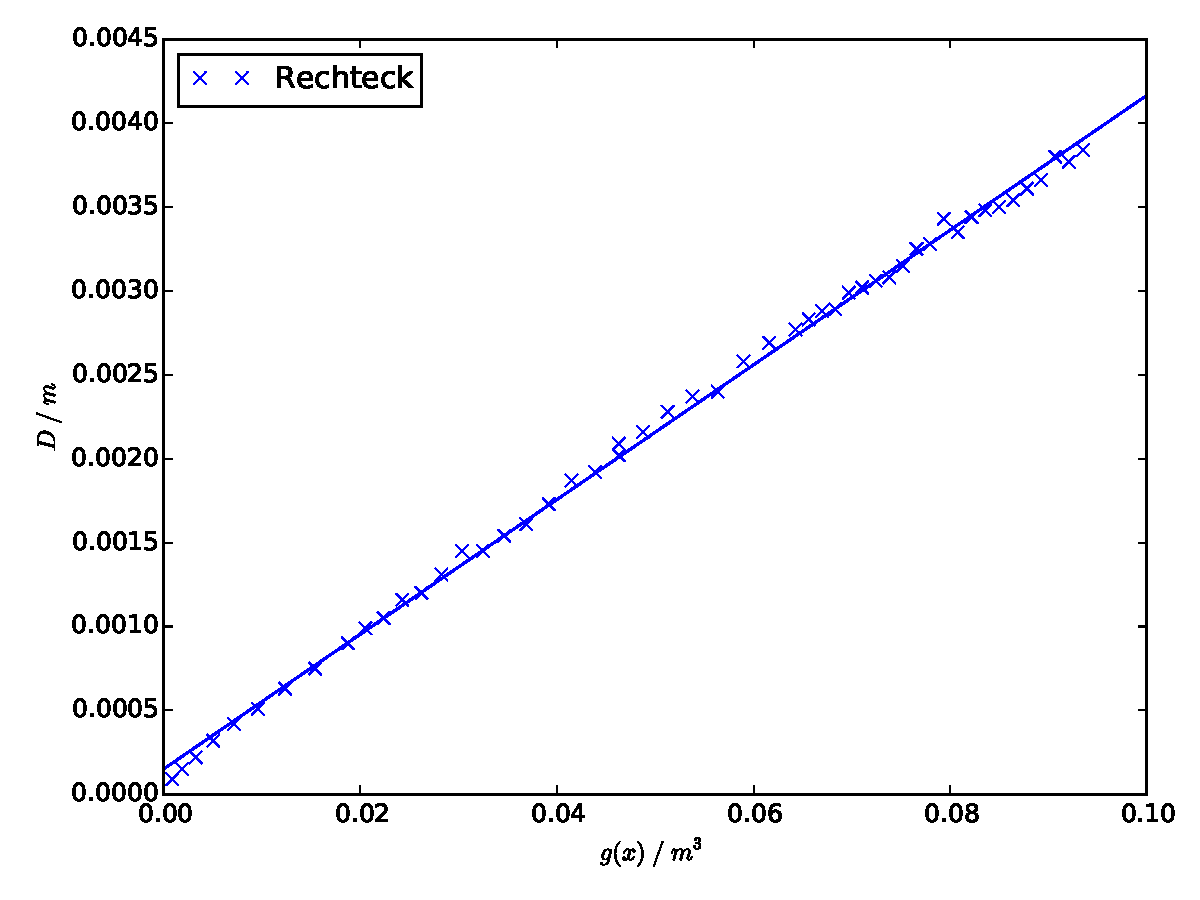
\includegraphics[width=\textwidth]{~/Documents/Uni/protokolle/Protokolle/Biegung_elastischer_Stäbe/Auswertung/plot1.pdf}
  \caption{Ausgleichskurve durch Messwerte des rechteckigen Stabes}
  \label{fig:kurveRecht}
\end{figure}


\begin{table}
  \centering
  \caption{Messdaten zum zylindrischen Stab}
  \label{tab:Zylwerte}
  \begin{tabular}{c c c c c c}
    \toprule
      $x\:/\:\si{\milli\meter}$ & $D_1\:/\:\si{\milli\meter}$ & $D_2\:/\:\si{\milli\meter}$ & $D(x)\:/\:\si{\milli\meter}$ & $g(x)=Lx^2-\frac{x^3}{3}$ \\
    \midrule
    505 & 6.52 & 1.52 & 5.00 & 9.09 \\
    500 & 6.57 & 1.62 & 4.95 & 8.95 \\
    495 & 6.51 & 1.73 & 4.78 & 8.82 \\
    490 & 6.60 & 1.78 & 4.82 & 8.68 \\
    485 & 6.65 & 1.93 & 4.71 & 8.54 \\
    480 & 6.63 & 2.05 & 4.58 & 8.40 \\
    475 & 6.64 & 2.11 & 4.53 & 8.27 \\
    470 & 6.75 & 2.22 & 4.53 & 8.13 \\
    465 & 6.70 & 2.30 & 4.40 & 8.00 \\
    460 & 6.74 & 2.32 & 4.41 & 7.86 \\
    455 & 6.76 & 2.45 & 4.31 & 7.72 \\
    450 & 6.82 & 2.69 & 4.12 & 7.59 \\
    445 & 6.86 & 2.72 & 4.13 & 7.45 \\
    440 & 6.89 & 2.83 & 4.06 & 7.32 \\
    435 & 6.92 & 2.90 & 4.02 & 7.19 \\
    430 & 6.97 & 2.98 & 3.99 & 7.05 \\
    425 & 6.94 & 3.07 & 3.87 & 6.92 \\
    420 & 6.96 & 3.18 & 3.78 & 6.79 \\
    415 & 6.99 & 3.29 & 3.70 & 6.65 \\
    410 & 7.03 & 3.38 & 3.64 & 6.52 \\
    405 & 7.06 & 3.43 & 3.62 & 6.39 \\
    400 & 7.11 & 3.59 & 3.52 & 6.26 \\
    395 & 7.12 & 3.66 & 3.45 & 6.13 \\
    390 & 7.15 & 3.74 & 3.41 & 6.00 \\
    385 & 7.16 & 3.82 & 3.33 & 5.87 \\
    380 & 7.19 & 3.90 & 3.29 & 5.75 \\
    370 & 8.75 & 5.62 & 3.12 & 5.49 \\
    360 & 8.72 & 5.79 & 2.93 & 5.24 \\
    350 & 8.79 & 5.93 & 2.85 & 5.00 \\
    340 & 8.83 & 6.10 & 2.72 & 4.75 \\
    330 & 8.83 & 6.27 & 2.56 & 4.51 \\
    320 & 8.85 & 6.41 & 2.43 & 4.28 \\
    310 & 8.91 & 6.55 & 2.35 & 4.05 \\
    300 & 8.89 & 6.68 & 2.20 & 3.82 \\
    290 & 8.91 & 6.78 & 2.12 & 3.60 \\
    280 & 8.96 & 6.96 & 2.00 & 3.38 \\
    270 & 9.00 & 7.14 & 1.86 & 3.17 \\
    260 & 9.02 & 7.28 & 1.73 & 2.96 \\
    250 & 9.04 & 7.39 & 1.65 & 2.76 \\
    240 & 9.05 & 7.50 & 1.55 & 2.56 \\
    230 & 9.09 & 7.62 & 1.46 & 2.37 \\
    220 & 9.08 & 7.73 & 1.35 & 2.18 \\
    210 & 9.08 & 7.85 & 1.22 & 2.00 \\
    200 & 9.10 & 7.95 & 1.15 & 1.83 \\
    180 & 9.11 & 8.16 & 0.95 & 1.50 \\
    160 & 9.11 & 8.32 & 0.79 & 1.20 \\
    140 & 9.12 & 8.49 & 0.63 & 0.93 \\
    120 & 9.11 & 8.62 & 0.48 & 0.69 \\
    100 & 9.11 & 8.74 & 0.36 & 0.49 \\
    80 & 9.09 & 8.83 & 0.26 & 0.31 \\
    60 & 9.09 & 8.92 & 0.17 & 0.18 \\
    \bottomrule
  \end{tabular}
\end{table}

\begin{figure}
  \centering
  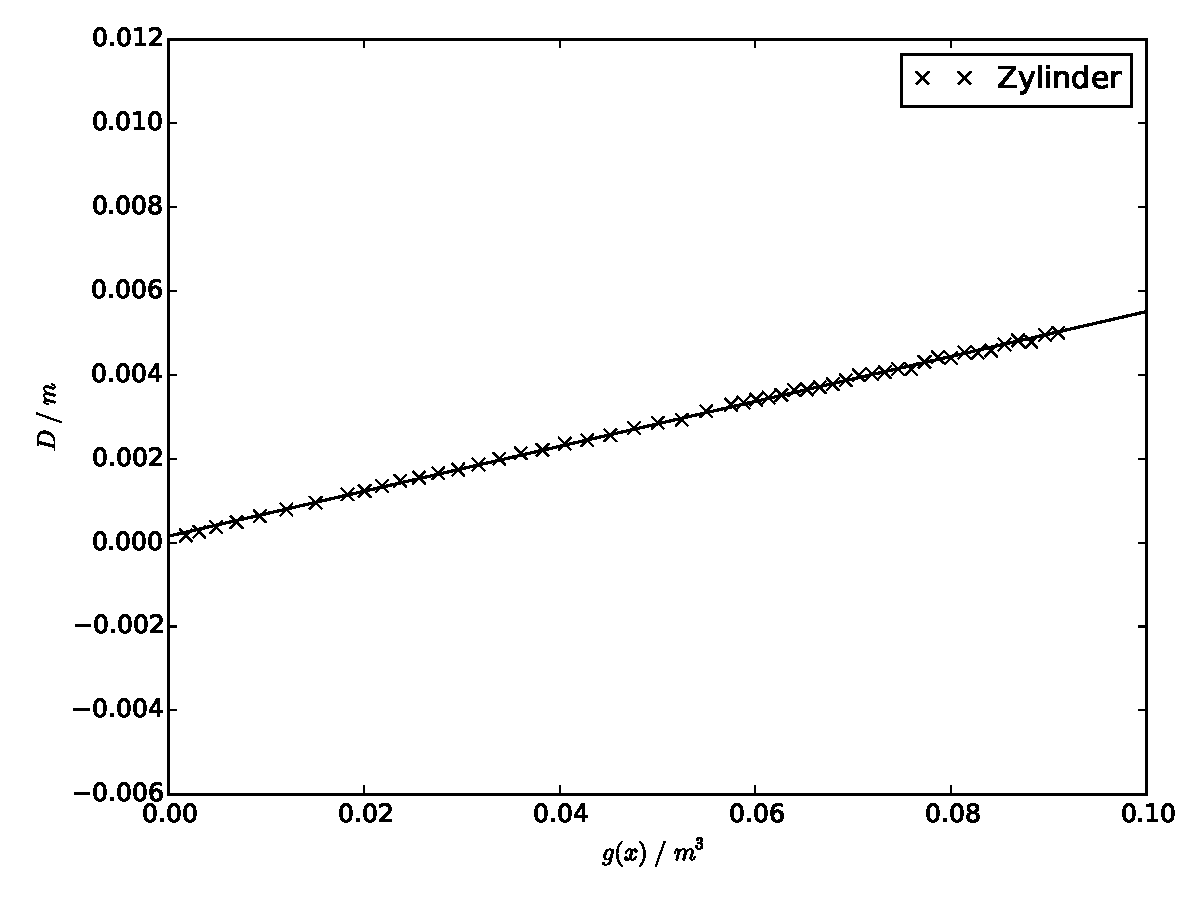
\includegraphics[width=\textwidth]{~/Documents/Uni/protokolle/Protokolle/Biegung_elastischer_Stäbe/Auswertung/plot2.pdf}
  \caption{Ausgleichskurve durch Messwerte des zylindrischen Stabes}
  \label{fig:kurveZyl}
\end{figure}


\begin{table}
  \centering
  \caption{Messdaten zum zweiseitig eingespannten rechteckigen Stab. Linke Seite}
  \label{tab:zweiwerte}
  \begin{tabular}{c c c c c c}
    \toprule
      $x\:/\:\si{\milli\meter}$ & $D_1\:/\:\si{\milli\meter}$ & $D_2\:/\:\si{\milli\meter}$ & $D(x)\:/\:\si{\milli\meter}$ & $(x)=Lx^2-\frac{x^3}{3}$ \\
    \midrule
      290 & 8.31 & 7.72  & 5.89 & 3.83 \\
      295 & 8.31 & 7.74  & 5.70 & 3.95 \\
      300 & 8.33 & 7.74  & 5.89 & 4.07 \\
      305 & 8.31 & 7.73  & 5.80 & 4.19 \\
      310 & 8.31 & 7.72  & 5.89 & 4.32 \\
      315 & 8.33 & 7.72  & 6.09 & 4.44 \\
      320 & 8.32 & 7.78  & 5.40 & 4.57 \\
      325 & 8.32 & 7.78  & 5.40 & 4.69 \\
      330 & 8.31 & 7.79  & 5.20 & 4.82 \\
      335 & 8.32 & 7.79  & 5.29 & 4.95 \\
      340 & 8.32 & 7.80  & 5.20 & 5.08 \\
      345 & 8.32 & 7.81  & 5.10 & 5.21 \\
      350 & 8.31 & 7.82  & 4.89 & 5.34 \\
      355 & 8.33 & 7.83  & 5.00 & 5.47 \\
      360 & 8.33 & 7.84  & 4.89 & 5.61 \\
      370 & 8.33 & 7.87  & 4.60 & 5.88 \\
      380 & 8.34 & 7.89  & 4.49 & 6.15 \\
      390 & 8.35 & 7.93  & 4.19 & 6.43 \\
      400 & 8.36 & 7.96  & 4.00 & 6.71 \\
      420 & 8.37 & 7.99  & 3.80 & 7.28 \\
      440 & 8.40 & 8.09  & 3.09 & 7.86 \\
      460 & 8.41 & 8.13  & 2.80 & 8.45 \\
      480 & 8.43 & 8.20  & 2.30 & 9.05 \\
      500 & 8.46 & 8.30  & 1.60 & 9.65 \\
      520 & 8.47 & 8.36  & 1.10 & 10.26 \\
    \bottomrule
  \end{tabular}
\end{table}

\begin{figure}
  \centering
  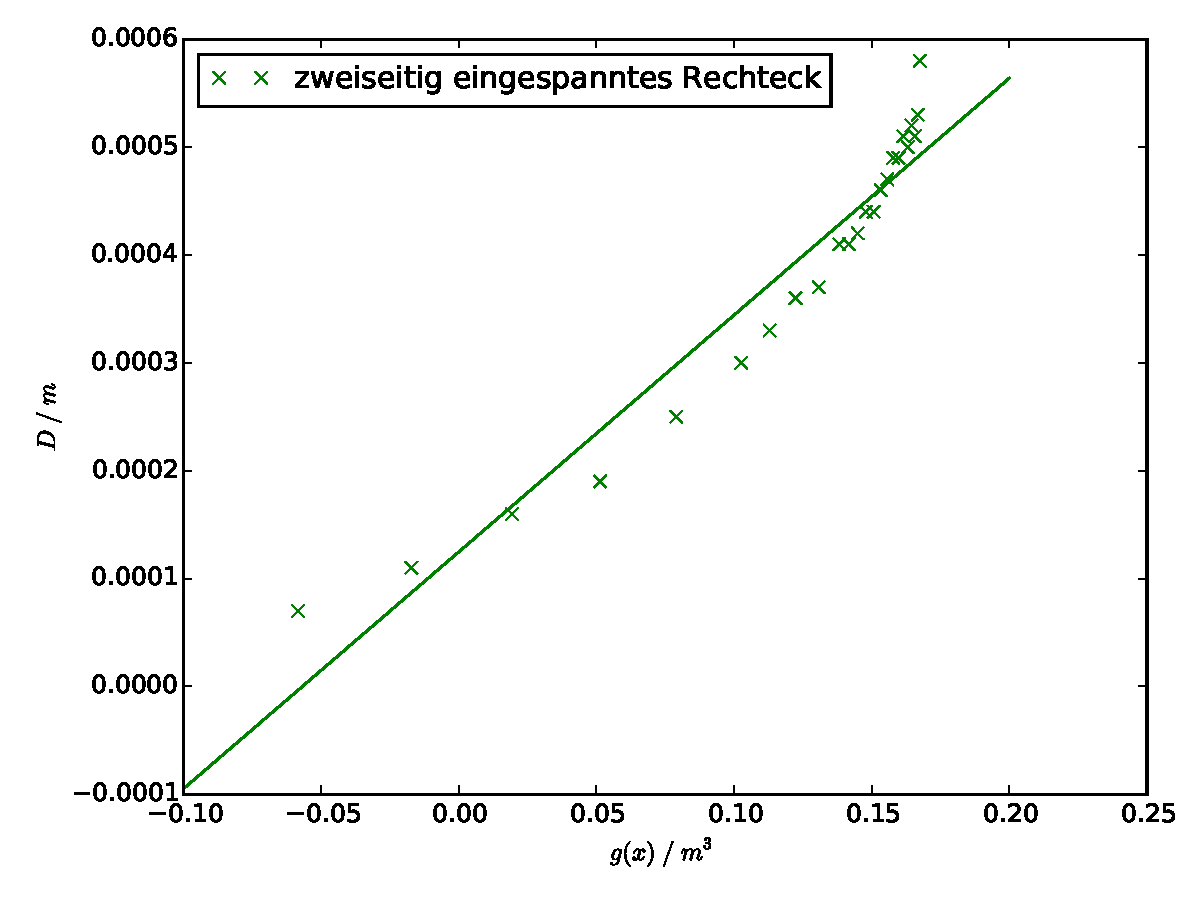
\includegraphics[width=\textwidth]{~/Documents/Uni/protokolle/Protokolle/Biegung_elastischer_Stäbe/Auswertung/plot4.pdf}
  \caption{Ausgleichskurve durch Messwerte des rechteckigen Stabes bei zweiseitiger Einspannung. Linke Seite.}
  \label{fig:kurveRechtlinks}
\end{figure}


\begin{table}
  \centering
  \caption{Messdaten zum zweiseitig eingespannten rechteckigen Stab. Rechte Seite}
  \label{tab:zweiwerte}
  \begin{tabular}{c c c c c c}
    \toprule
      $x\:/\:\si{\milli\meter}$ & $D_1\:/\:\si{\milli\meter}$ & $D_2\:/\:\si{\milli\meter}$ & $D(x)\:/\:\si{\milli\meter}$ & $g(x)=Lx^2-\frac{x^3}{3}$ \\
    \midrule
    255 & 10.08 & 9.50 & 5.80 & 3.04 \\
    250 & 10.08 & 9.55 & 5.29 & 2.93 \\
    245 & 10.07 & 9.56 & 5.10 & 2.82 \\
    240 & 10.09 & 9.57 & 5.20 & 2.72 \\
    235 & 10.08 & 9.58 & 5.00 & 2.62 \\
    230 & 10.11 & 9.60 & 5.10 & 2.51 \\
    225 & 10.11 & 9.62 & 4.89 & 2.41 \\
    220 & 10.13 & 9.64 & 4.89 & 2.32 \\
    215 & 10.13 & 9.66 & 4.70 & 2.22 \\
    210 & 10.15 & 9.69 & 4.60 & 2.13 \\
    205 & 10.16 & 9.72 & 4.40 & 2.03 \\
    200 & 10.17 & 9.73 & 4.40 & 1.94 \\
    195 & 10.18 & 9.76 & 4.19 & 1.85 \\
    190 & 10.20 & 9.79 & 4.10 & 1.76 \\
    185 & 10.21 & 9.80 & 4.10 & 1.68 \\
    175 & 10.23 & 9.86 & 3.69 & 1.51 \\
    165 & 10.26 & 9.90 & 3.59 & 1.35 \\
    155 & 10.30 & 9.97 & 3.29 & 1.20 \\
    145 & 10.32 & 10.02 & 2.99 & 1.06 \\
    125 & 10.40 & 10.15 & 2.50 & 0.79 \\
    105 & 10.45 & 10.26 & 1.90 & 0.57 \\
    85 & 10.54 & 10.38 & 1.60 & 0.37 \\
    65 & 10.62 & 10.51 & 1.10 & 0.22 \\
    45 & 10.69 & 10.62 & 0.70 & 0.10 \\
    \bottomrule
  \end{tabular}
\end{table}

\begin{figure}
  \centering
  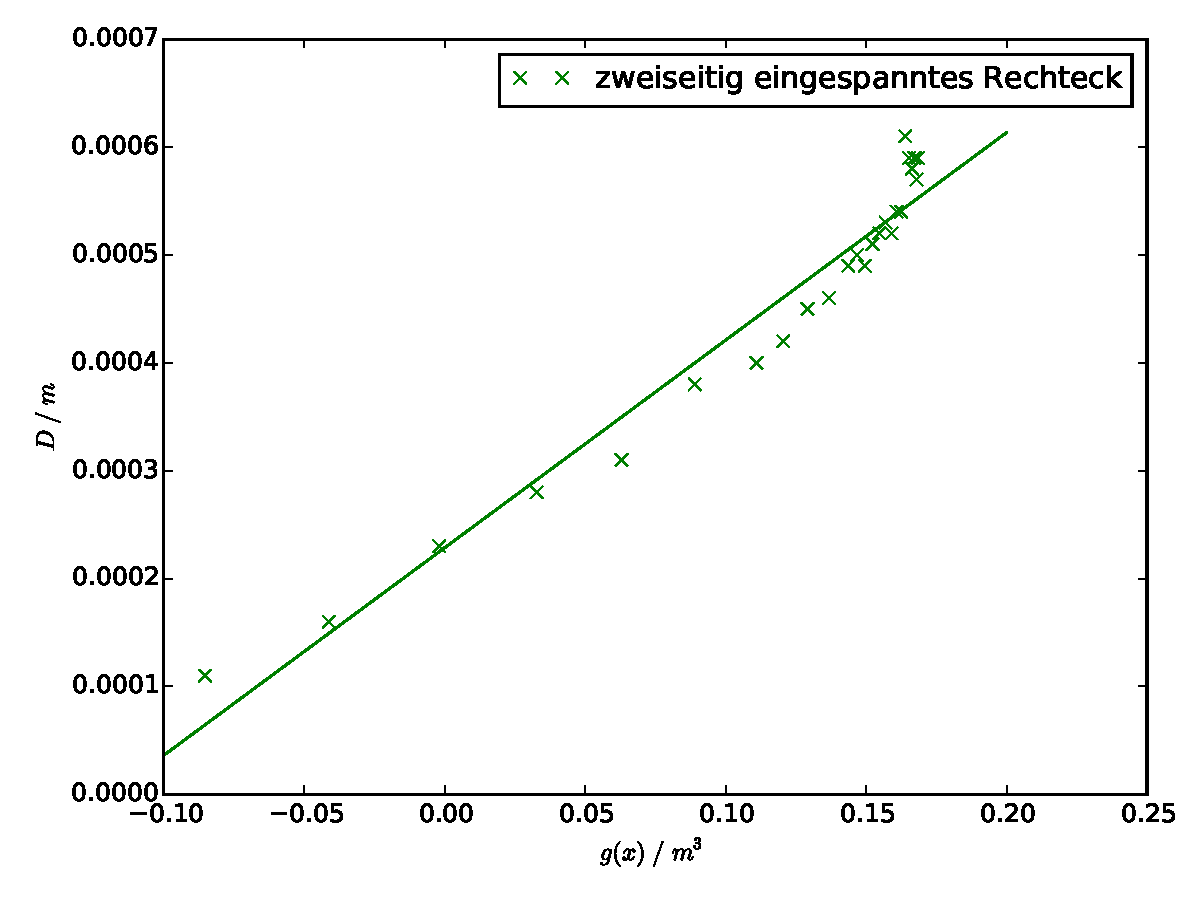
\includegraphics[width=\textwidth]{~/Documents/Uni/protokolle/Protokolle/Biegung_elastischer_Stäbe/Auswertung/plot3.pdf}
  \caption{Ausgleichskurve durch Messwerte des rechteckigen Stabes. Rechte Seite.}
  \label{fig:kurveRechtrechts}
\end{figure}
